Debido a la complejidad de las aplicaciones web modernas, es necesario 
realizar una serie de pasos intermedios entre el código original y 
el resultado final de la apliación. Para el caso de este proyecto, se debe:

\begin{itemize}

\item Compilar el código typescript a javascript.

\item Compilar el código .tsx a .jsx.

\item Resolver las importaciones de dependencias, tanto de la lógica
como de los componentes.

\item Procesar el código sass y convertirlo en css.

\end{itemize}

\subsection{Gulp/Grunt}

La primera tendencia -debido a su gran extensión- sería utilizar 
lo que se conoce como un \textit{task runner}. Actualmente, dos de los 
más conocidos son \textbf{Gulp} y \textbf{Grunt}.

\bigskip
Ambos están basados en NodeJs y son compatibles entre sí en gran medida.
Su funcionamiento es sencillo, en un gruntfile o gulpfile se definen las tareas a
ejecutar, seleccionando los ficheros de fuente sobre los que actuar -si cabe- y la tarea 
a realizar.

\bigskip
Existen muchisimos plugins desarrollados que permiten hacer todo tipo de tareas, desde traducir
markdown hasta minimizar el contenido de los ficheros de estilos y de javascript.

\bigskip
Sin embargo, a pesar de que esta opción era altamente atractiva debido 
a su robustez, se ha optado por probar una solución aún más moderna, \textbf{webpack}.

\subsection{Webpack}

Webpack es un \textit{empaquetador de módulos} para aplicaciones de Javascript modernas.
Cuando webpack procesa la aplicación, construye un grafo de dependencias
incluyendo todos los módulos y luego lo empaqueta en orden. 

\bigskip
Webpack posee de forma intrínseca diversas características interensantes tales como el 
poder ejecutar un servidor de desarrollo que aplica \textit{hot reloading} sobr el código 
sin requerir refrescar la página o el poder separar el código css/js de terceros para el 
entorno de producción. 

\bigskip 
El funcionamiento de webpack puede ser extremadamente resumido y simplificado en:

\begin{itemize}

\item Partiendo de un punto de entrada, una serie de reglas sobre los distintos tipos de ficheros
activan una serie de \textit{loaders} correspondientes para procesarlos. 

\item Estos loaders pueden ser concatenados entre sí para obtener el resultado deseado, por ejemplo
podemos traducir el código typescript a es6 para luego traducir este código junto a otro a es5 mediante
babel.

\item Se aplican, si fuera necesario, el uso de plugins para tareas más complejas que se quieren aplicar sobre
todos los paquetes.

\end{itemize}

\begin{figure}[!th]
\begin{center}
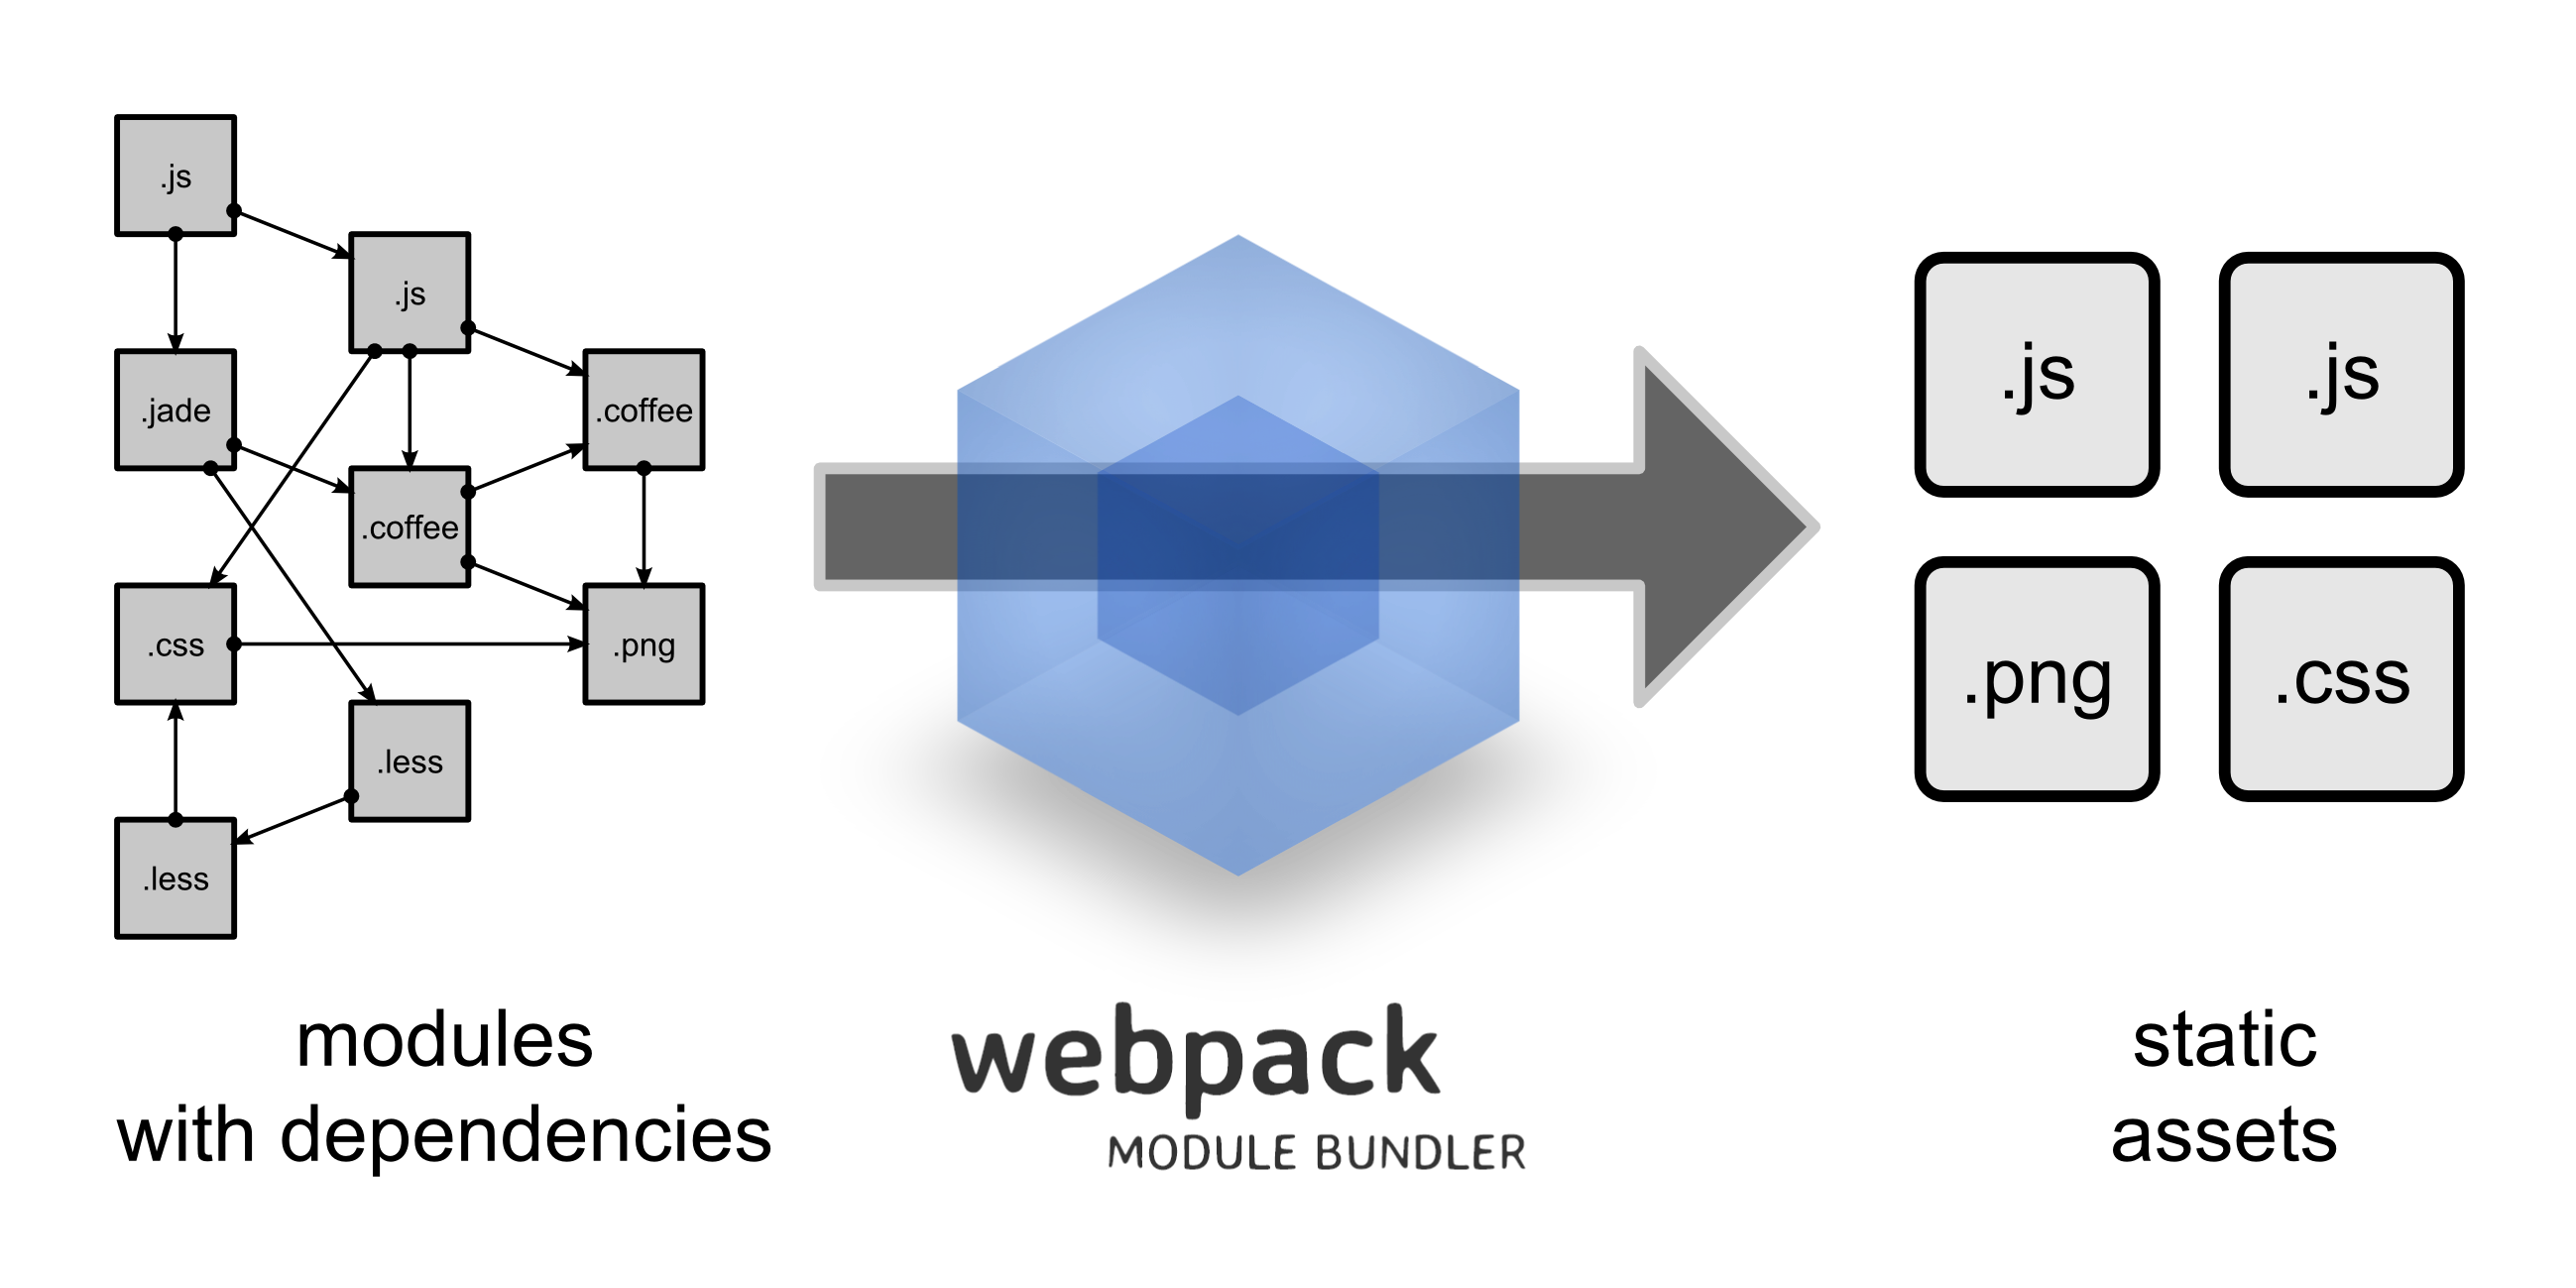
\includegraphics[width=0.8\textwidth]{images/cap4/webpack.eps}
\caption{Imagen descriptiva de Webpack}
\label{fig:Imagen descriptiva de Webpack}
\end{center}
\end{figure}


Como resultado final se obtiene una serie de paquetes que contienen todas las dependencias resueltas.